\documentclass[]{article}
\usepackage{lmodern}
\usepackage{amssymb,amsmath}
\usepackage{ifxetex,ifluatex}
\usepackage{fixltx2e} % provides \textsubscript
\ifnum 0\ifxetex 1\fi\ifluatex 1\fi=0 % if pdftex
  \usepackage[T1]{fontenc}
  \usepackage[utf8]{inputenc}
\else % if luatex or xelatex
  \ifxetex
    \usepackage{mathspec}
  \else
    \usepackage{fontspec}
  \fi
  \defaultfontfeatures{Ligatures=TeX,Scale=MatchLowercase}
\fi
% use upquote if available, for straight quotes in verbatim environments
\IfFileExists{upquote.sty}{\usepackage{upquote}}{}
% use microtype if available
\IfFileExists{microtype.sty}{%
\usepackage{microtype}
\UseMicrotypeSet[protrusion]{basicmath} % disable protrusion for tt fonts
}{}
\usepackage[margin=1in]{geometry}
\usepackage{hyperref}
\hypersetup{unicode=true,
            pdftitle={Final Project- Exploring Temperatures in California Between 1989-2018},
            pdfauthor={Chauncey Quam},
            pdfborder={0 0 0},
            breaklinks=true}
\urlstyle{same}  % don't use monospace font for urls
\usepackage{color}
\usepackage{fancyvrb}
\newcommand{\VerbBar}{|}
\newcommand{\VERB}{\Verb[commandchars=\\\{\}]}
\DefineVerbatimEnvironment{Highlighting}{Verbatim}{commandchars=\\\{\}}
% Add ',fontsize=\small' for more characters per line
\usepackage{framed}
\definecolor{shadecolor}{RGB}{248,248,248}
\newenvironment{Shaded}{\begin{snugshade}}{\end{snugshade}}
\newcommand{\AlertTok}[1]{\textcolor[rgb]{0.94,0.16,0.16}{#1}}
\newcommand{\AnnotationTok}[1]{\textcolor[rgb]{0.56,0.35,0.01}{\textbf{\textit{#1}}}}
\newcommand{\AttributeTok}[1]{\textcolor[rgb]{0.77,0.63,0.00}{#1}}
\newcommand{\BaseNTok}[1]{\textcolor[rgb]{0.00,0.00,0.81}{#1}}
\newcommand{\BuiltInTok}[1]{#1}
\newcommand{\CharTok}[1]{\textcolor[rgb]{0.31,0.60,0.02}{#1}}
\newcommand{\CommentTok}[1]{\textcolor[rgb]{0.56,0.35,0.01}{\textit{#1}}}
\newcommand{\CommentVarTok}[1]{\textcolor[rgb]{0.56,0.35,0.01}{\textbf{\textit{#1}}}}
\newcommand{\ConstantTok}[1]{\textcolor[rgb]{0.00,0.00,0.00}{#1}}
\newcommand{\ControlFlowTok}[1]{\textcolor[rgb]{0.13,0.29,0.53}{\textbf{#1}}}
\newcommand{\DataTypeTok}[1]{\textcolor[rgb]{0.13,0.29,0.53}{#1}}
\newcommand{\DecValTok}[1]{\textcolor[rgb]{0.00,0.00,0.81}{#1}}
\newcommand{\DocumentationTok}[1]{\textcolor[rgb]{0.56,0.35,0.01}{\textbf{\textit{#1}}}}
\newcommand{\ErrorTok}[1]{\textcolor[rgb]{0.64,0.00,0.00}{\textbf{#1}}}
\newcommand{\ExtensionTok}[1]{#1}
\newcommand{\FloatTok}[1]{\textcolor[rgb]{0.00,0.00,0.81}{#1}}
\newcommand{\FunctionTok}[1]{\textcolor[rgb]{0.00,0.00,0.00}{#1}}
\newcommand{\ImportTok}[1]{#1}
\newcommand{\InformationTok}[1]{\textcolor[rgb]{0.56,0.35,0.01}{\textbf{\textit{#1}}}}
\newcommand{\KeywordTok}[1]{\textcolor[rgb]{0.13,0.29,0.53}{\textbf{#1}}}
\newcommand{\NormalTok}[1]{#1}
\newcommand{\OperatorTok}[1]{\textcolor[rgb]{0.81,0.36,0.00}{\textbf{#1}}}
\newcommand{\OtherTok}[1]{\textcolor[rgb]{0.56,0.35,0.01}{#1}}
\newcommand{\PreprocessorTok}[1]{\textcolor[rgb]{0.56,0.35,0.01}{\textit{#1}}}
\newcommand{\RegionMarkerTok}[1]{#1}
\newcommand{\SpecialCharTok}[1]{\textcolor[rgb]{0.00,0.00,0.00}{#1}}
\newcommand{\SpecialStringTok}[1]{\textcolor[rgb]{0.31,0.60,0.02}{#1}}
\newcommand{\StringTok}[1]{\textcolor[rgb]{0.31,0.60,0.02}{#1}}
\newcommand{\VariableTok}[1]{\textcolor[rgb]{0.00,0.00,0.00}{#1}}
\newcommand{\VerbatimStringTok}[1]{\textcolor[rgb]{0.31,0.60,0.02}{#1}}
\newcommand{\WarningTok}[1]{\textcolor[rgb]{0.56,0.35,0.01}{\textbf{\textit{#1}}}}
\usepackage{graphicx,grffile}
\makeatletter
\def\maxwidth{\ifdim\Gin@nat@width>\linewidth\linewidth\else\Gin@nat@width\fi}
\def\maxheight{\ifdim\Gin@nat@height>\textheight\textheight\else\Gin@nat@height\fi}
\makeatother
% Scale images if necessary, so that they will not overflow the page
% margins by default, and it is still possible to overwrite the defaults
% using explicit options in \includegraphics[width, height, ...]{}
\setkeys{Gin}{width=\maxwidth,height=\maxheight,keepaspectratio}
\IfFileExists{parskip.sty}{%
\usepackage{parskip}
}{% else
\setlength{\parindent}{0pt}
\setlength{\parskip}{6pt plus 2pt minus 1pt}
}
\setlength{\emergencystretch}{3em}  % prevent overfull lines
\providecommand{\tightlist}{%
  \setlength{\itemsep}{0pt}\setlength{\parskip}{0pt}}
\setcounter{secnumdepth}{0}
% Redefines (sub)paragraphs to behave more like sections
\ifx\paragraph\undefined\else
\let\oldparagraph\paragraph
\renewcommand{\paragraph}[1]{\oldparagraph{#1}\mbox{}}
\fi
\ifx\subparagraph\undefined\else
\let\oldsubparagraph\subparagraph
\renewcommand{\subparagraph}[1]{\oldsubparagraph{#1}\mbox{}}
\fi

%%% Use protect on footnotes to avoid problems with footnotes in titles
\let\rmarkdownfootnote\footnote%
\def\footnote{\protect\rmarkdownfootnote}

%%% Change title format to be more compact
\usepackage{titling}

% Create subtitle command for use in maketitle
\newcommand{\subtitle}[1]{
  \posttitle{
    \begin{center}\large#1\end{center}
    }
}

\setlength{\droptitle}{-2em}

  \title{Final Project- Exploring Temperatures in California Between 1989-2018}
    \pretitle{\vspace{\droptitle}\centering\huge}
  \posttitle{\par}
    \author{Chauncey Quam}
    \preauthor{\centering\large\emph}
  \postauthor{\par}
      \predate{\centering\large\emph}
  \postdate{\par}
    \date{11/10/2019}


\begin{document}
\maketitle

setwd

\#\#Load Packages needed for data analysis.

\begin{Shaded}
\begin{Highlighting}[]
\CommentTok{# install.packages("tidyverse")}
\CommentTok{# install.packages("tidyr")}
\CommentTok{# install.packages("readxl")}
\CommentTok{# install.packages("dplyr")}
\CommentTok{# install.packages("lubridate")}
\CommentTok{# install.packages("ggplot2")}
\CommentTok{# install.packages("maps")}
\CommentTok{# install.packages('tinytex')}
\KeywordTok{library}\NormalTok{(}\StringTok{"tidyverse"}\NormalTok{)}
\end{Highlighting}
\end{Shaded}

\begin{verbatim}
## Warning: package 'tidyverse' was built under R version 3.5.2
\end{verbatim}

\begin{verbatim}
## ── Attaching packages ───────────────────────────────────────────────────────────────── tidyverse 1.3.0 ──
\end{verbatim}

\begin{verbatim}
## ✓ ggplot2 3.2.1     ✓ purrr   0.3.3
## ✓ tibble  2.1.3     ✓ dplyr   0.8.3
## ✓ tidyr   1.0.0     ✓ stringr 1.4.0
## ✓ readr   1.3.1     ✓ forcats 0.4.0
\end{verbatim}

\begin{verbatim}
## Warning: package 'ggplot2' was built under R version 3.5.2
\end{verbatim}

\begin{verbatim}
## Warning: package 'tibble' was built under R version 3.5.2
\end{verbatim}

\begin{verbatim}
## Warning: package 'tidyr' was built under R version 3.5.2
\end{verbatim}

\begin{verbatim}
## Warning: package 'purrr' was built under R version 3.5.2
\end{verbatim}

\begin{verbatim}
## Warning: package 'dplyr' was built under R version 3.5.2
\end{verbatim}

\begin{verbatim}
## Warning: package 'stringr' was built under R version 3.5.2
\end{verbatim}

\begin{verbatim}
## Warning: package 'forcats' was built under R version 3.5.2
\end{verbatim}

\begin{verbatim}
## ── Conflicts ──────────────────────────────────────────────────────────────────── tidyverse_conflicts() ──
## x dplyr::filter() masks stats::filter()
## x dplyr::lag()    masks stats::lag()
\end{verbatim}

\begin{Shaded}
\begin{Highlighting}[]
\KeywordTok{library}\NormalTok{(}\StringTok{"readxl"}\NormalTok{)}
\end{Highlighting}
\end{Shaded}

\begin{verbatim}
## Warning: package 'readxl' was built under R version 3.5.2
\end{verbatim}

\begin{Shaded}
\begin{Highlighting}[]
\KeywordTok{library}\NormalTok{(}\StringTok{"dplyr"}\NormalTok{)}
\KeywordTok{library}\NormalTok{(}\StringTok{"lubridate"}\NormalTok{)}
\end{Highlighting}
\end{Shaded}

\begin{verbatim}
## 
## Attaching package: 'lubridate'
\end{verbatim}

\begin{verbatim}
## The following object is masked from 'package:base':
## 
##     date
\end{verbatim}

\begin{Shaded}
\begin{Highlighting}[]
\KeywordTok{library}\NormalTok{(}\StringTok{"ggplot2"}\NormalTok{)}
\KeywordTok{library}\NormalTok{(}\StringTok{"maps"}\NormalTok{)}
\end{Highlighting}
\end{Shaded}

\begin{verbatim}
## 
## Attaching package: 'maps'
\end{verbatim}

\begin{verbatim}
## The following object is masked from 'package:purrr':
## 
##     map
\end{verbatim}

\begin{Shaded}
\begin{Highlighting}[]
\KeywordTok{library}\NormalTok{(}\StringTok{'tinytex'}\NormalTok{)}
\end{Highlighting}
\end{Shaded}

\begin{verbatim}
## Warning: package 'tinytex' was built under R version 3.5.2
\end{verbatim}

\begin{Shaded}
\begin{Highlighting}[]
\CommentTok{#tinytex::install_tinytex()}
\end{Highlighting}
\end{Shaded}

\#In this project I will be examining daily temperature observations for
selected counties in California during the past 30 years. These counties
were selected because they are all major agricultural producing counties
in California. Extreme temperature can have a drastic effect on crop
yield. As climate in California changes our current agricultural
production regions of California might become less productive as
temperature increases. This project attempts to explore instances of
extreme temperatures, classified as temperatures of 105 degrees or
higher.

\#\#Reading Data Files \#\#\#I began this project by downloading
temperature data from the \href{https://www.climate.gov/maps-data}{NOAA
climate website}. I hand selected counties to request this data for. The
data files I received and am using in this project are daily temperature
observations from stations located within major agricultural producing
counties of California.

\#\#\#I loaded in data from the CSV files and created one table with all
of the temperature observation files.

\begin{Shaded}
\begin{Highlighting}[]
\NormalTok{df_}\DecValTok{1}\NormalTok{ <-}\StringTok{ }\KeywordTok{read_csv}\NormalTok{(}\StringTok{"CSV data files/1929501.csv"}\NormalTok{, }\DataTypeTok{col_types =} \KeywordTok{cols}\NormalTok{(}\DataTypeTok{TMAX =} \KeywordTok{col_integer}\NormalTok{(), }\DataTypeTok{TMIN =} \KeywordTok{col_integer}\NormalTok{()),}\DataTypeTok{col_names=}\OtherTok{TRUE}\NormalTok{)}
\NormalTok{df_}\DecValTok{2}\NormalTok{ <-}\StringTok{ }\KeywordTok{read_csv}\NormalTok{(}\StringTok{"CSV data files/1929502.csv"}\NormalTok{, }\DataTypeTok{col_types =} \KeywordTok{cols}\NormalTok{(}\DataTypeTok{TMAX =} \KeywordTok{col_integer}\NormalTok{(), }\DataTypeTok{TMIN =} \KeywordTok{col_integer}\NormalTok{()),}\DataTypeTok{col_names=}\OtherTok{TRUE}\NormalTok{)}
\NormalTok{df_}\DecValTok{3}\NormalTok{ <-}\StringTok{ }\KeywordTok{read_csv}\NormalTok{(}\StringTok{"CSV data files/1929482.csv"}\NormalTok{, }\DataTypeTok{col_types =} \KeywordTok{cols}\NormalTok{(}\DataTypeTok{TMAX =} \KeywordTok{col_integer}\NormalTok{(), }\DataTypeTok{TMIN =} \KeywordTok{col_integer}\NormalTok{()),}\DataTypeTok{col_names=}\OtherTok{TRUE}\NormalTok{)}
\NormalTok{df_}\DecValTok{4}\NormalTok{ <-}\StringTok{ }\KeywordTok{read_csv}\NormalTok{(}\StringTok{"CSV data files/1929489.csv"}\NormalTok{, }\DataTypeTok{col_types =} \KeywordTok{cols}\NormalTok{(}\DataTypeTok{TMAX =} \KeywordTok{col_integer}\NormalTok{(), }\DataTypeTok{TMIN =} \KeywordTok{col_integer}\NormalTok{()),}\DataTypeTok{col_names=}\OtherTok{TRUE}\NormalTok{)}
\NormalTok{df_}\DecValTok{5}\NormalTok{ <-}\StringTok{ }\KeywordTok{read_csv}\NormalTok{(}\StringTok{"CSV data files/1929497.csv"}\NormalTok{, }\DataTypeTok{col_types =} \KeywordTok{cols}\NormalTok{(}\DataTypeTok{TMAX =} \KeywordTok{col_integer}\NormalTok{(), }\DataTypeTok{TMIN =} \KeywordTok{col_integer}\NormalTok{()),}\DataTypeTok{col_names=}\OtherTok{TRUE}\NormalTok{)}

\NormalTok{all_data <-}\StringTok{ }\KeywordTok{rbind}\NormalTok{(df_}\DecValTok{1}\NormalTok{, df_}\DecValTok{2}\NormalTok{, df_}\DecValTok{3}\NormalTok{, df_}\DecValTok{4}\NormalTok{, df_}\DecValTok{5}\NormalTok{)}
\KeywordTok{head}\NormalTok{(all_data)}
\end{Highlighting}
\end{Shaded}

\begin{verbatim}
## # A tibble: 6 x 8
##   STATION   NAME        LATITUDE LONGITUDE ELEVATION DATE        TMAX  TMIN
##   <chr>     <chr>          <dbl>     <dbl>     <dbl> <date>     <int> <int>
## 1 US1CASR0… BARSTOW 0.…     34.9     -117.      795. 2010-01-22    NA    NA
## 2 US1CASR0… BARSTOW 0.…     34.9     -117.      795. 2010-01-27    NA    NA
## 3 US1CASR0… BARSTOW 0.…     34.9     -117.      795. 2010-02-06    NA    NA
## 4 US1CASR0… BARSTOW 0.…     34.9     -117.      795. 2010-02-07    NA    NA
## 5 US1CASR0… BARSTOW 0.…     34.9     -117.      795. 2010-02-10    NA    NA
## 6 US1CASR0… BARSTOW 0.…     34.9     -117.      795. 2010-02-28    NA    NA
\end{verbatim}

\#\#Cleaning Dataset \#\#\#I decided to omit all NA variables for
temperature using the code below.

\begin{Shaded}
\begin{Highlighting}[]
\NormalTok{all_data <-}\StringTok{ }\NormalTok{all_data[}\KeywordTok{complete.cases}\NormalTok{(all_data}\OperatorTok{$}\NormalTok{TMAX), ]}
\end{Highlighting}
\end{Shaded}

\#\#\#I seperated the full date into three columns by year, month, day.

\begin{Shaded}
\begin{Highlighting}[]
\NormalTok{all_data <-}\StringTok{ }\KeywordTok{separate}\NormalTok{(all_data,DATE, }\KeywordTok{c}\NormalTok{(}\StringTok{"YEAR"}\NormalTok{, }\StringTok{"MONTH"}\NormalTok{, }\StringTok{"DAY"}\NormalTok{),}\StringTok{"-"}\NormalTok{)}
\end{Highlighting}
\end{Shaded}

\#\#Isolating name of town. \#\#\#I am doing this by first taking the
names column and parcing into seperate columns, seperating by a space or
a comma. I then drop all added columns becides CITY.

\begin{Shaded}
\begin{Highlighting}[]
\NormalTok{all_data <-}\StringTok{ }\KeywordTok{separate}\NormalTok{(all_data, NAME, }\KeywordTok{c}\NormalTok{(}\StringTok{"CITY"}\NormalTok{,}\StringTok{"STATE"}\NormalTok{,}\StringTok{"COUNTRY"}\NormalTok{, }\StringTok{"x1"}\NormalTok{, }\StringTok{"x2"}\NormalTok{, }\StringTok{"x3"}\NormalTok{, }\StringTok{"x4"}\NormalTok{), }
    \DataTypeTok{sep =} \StringTok{"([}\CharTok{\textbackslash{}\textbackslash{}}\StringTok{ }\CharTok{\textbackslash{}\textbackslash{}}\StringTok{,])"}\NormalTok{)}
\end{Highlighting}
\end{Shaded}

\begin{verbatim}
## Warning: Expected 7 pieces. Missing pieces filled with `NA` in 221976
## rows [1, 2, 3, 4, 5, 6, 7, 8, 9, 10, 11, 12, 13, 14, 15, 16, 17, 18, 19,
## 20, ...].
\end{verbatim}

\begin{Shaded}
\begin{Highlighting}[]
\NormalTok{all_data <-}\StringTok{ }\NormalTok{all_data }\OperatorTok
\StringTok{  }\KeywordTok{select}\NormalTok{(}\OperatorTok{-}\KeywordTok{c}\NormalTok{(STATE, COUNTRY,x1,x2,x3,x4)) }
\CommentTok{# subset(all_data, select = -c(STATE, COUNTRY,x1,x2,x3,x4))}
\CommentTok{# all_data <- unite(all_data, CITY, select =CITY, sep = " ")}
\KeywordTok{head}\NormalTok{(all_data)}
\end{Highlighting}
\end{Shaded}

\begin{verbatim}
## # A tibble: 6 x 10
##   STATION  CITY  LATITUDE LONGITUDE ELEVATION YEAR  MONTH DAY    TMAX  TMIN
##   <chr>    <chr>    <dbl>     <dbl>     <dbl> <chr> <chr> <chr> <int> <int>
## 1 USC0004… BLYT…     33.6     -115.      81.7 1989  01    01       61    NA
## 2 USC0004… BLYT…     33.6     -115.      81.7 1989  01    02       65    28
## 3 USC0004… BLYT…     33.6     -115.      81.7 1989  01    03       65    40
## 4 USC0004… BLYT…     33.6     -115.      81.7 1989  01    04       64    49
## 5 USC0004… BLYT…     33.6     -115.      81.7 1989  01    05       65    39
## 6 USC0004… BLYT…     33.6     -115.      81.7 1989  01    06       55    40
\end{verbatim}

\#\#\#Check to see what every city name is.

\begin{Shaded}
\begin{Highlighting}[]
\KeywordTok{unique}\NormalTok{(all_data}\OperatorTok{$}\NormalTok{CITY) }
\end{Highlighting}
\end{Shaded}

\begin{verbatim}
##  [1] "BLYTHE"     "SQUAW"      "GOLD"       "PICACHO"    "BARSTOW"   
##  [6] "IMPERIAL"   "LORAINE"    "CAHUILLA"   "BUTTERCUP"  "HOLLISTER" 
## [11] "PAICINES"   "RED"        "WOODLAND"   "CHICO"      "LINCOLN"   
## [16] "STOCKTON"   "TRACY"      "STONYFORD"  "PETALUMA"   "SACRAMENTO"
## [21] "EAST"       "HANFORD"    "DELANO"     "COALINGA"   "MERCED"
\end{verbatim}

\#\#\#I have selected only the first word for each town name. I will now
add the words that were omitted from town names manually so that town
names are complete in the dataset.

\begin{Shaded}
\begin{Highlighting}[]
\NormalTok{id <-}\StringTok{ }\KeywordTok{c}\NormalTok{(}\StringTok{"SQUAW"}\NormalTok{, }\StringTok{"GOLD"}\NormalTok{, }\StringTok{"IMPERIAL"}\NormalTok{, }\StringTok{"RED"}\NormalTok{, }\StringTok{"EAST"}\NormalTok{)}
\NormalTok{names<-}\StringTok{ }\KeywordTok{c}\NormalTok{(}\StringTok{"SQUAW LAKE"}\NormalTok{, }\StringTok{"GOLD ROCK RANCH"}\NormalTok{, }\StringTok{"IMPERIAL SAND DUNES"}\NormalTok{, }\StringTok{"RED BLUFF"}\NormalTok{, }\StringTok{"EAST PARK RESERVOIR"}\NormalTok{)}

\ControlFlowTok{for}\NormalTok{ (i }\ControlFlowTok{in} \KeywordTok{c}\NormalTok{(}\DecValTok{1}\OperatorTok{:}\KeywordTok{length}\NormalTok{(id))) \{}
\NormalTok{  all_data}\OperatorTok{$}\NormalTok{CITY <-}\StringTok{ }\KeywordTok{ifelse}\NormalTok{(all_data}\OperatorTok{$}\NormalTok{CITY }\OperatorTok{==}\StringTok{ }\NormalTok{id[i],}
                          \DataTypeTok{yes =}\NormalTok{ names[i],}
                          \DataTypeTok{no =}\NormalTok{ all_data}\OperatorTok{$}\NormalTok{CITY)}
\NormalTok{\}}
\KeywordTok{unique}\NormalTok{(all_data}\OperatorTok{$}\NormalTok{CITY)}
\end{Highlighting}
\end{Shaded}

\begin{verbatim}
##  [1] "BLYTHE"              "SQUAW LAKE"          "GOLD ROCK RANCH"    
##  [4] "PICACHO"             "BARSTOW"             "IMPERIAL SAND DUNES"
##  [7] "LORAINE"             "CAHUILLA"            "BUTTERCUP"          
## [10] "HOLLISTER"           "PAICINES"            "RED BLUFF"          
## [13] "WOODLAND"            "CHICO"               "LINCOLN"            
## [16] "STOCKTON"            "TRACY"               "STONYFORD"          
## [19] "PETALUMA"            "SACRAMENTO"          "EAST PARK RESERVOIR"
## [22] "HANFORD"             "DELANO"              "COALINGA"           
## [25] "MERCED"
\end{verbatim}

\#\#\#I also notice that there are some cities that have two observation
stations reporting data. I remove these double counts so as not to bias
my results.

\begin{Shaded}
\begin{Highlighting}[]
\NormalTok{all_data <-}\StringTok{ }\NormalTok{all_data }\OperatorTok
\StringTok{       }\KeywordTok{distinct}\NormalTok{(CITY,YEAR,MONTH,DAY, }\DataTypeTok{.keep_all =} \OtherTok{TRUE}\NormalTok{)}
\KeywordTok{nrow}\NormalTok{(all_data)}
\end{Highlighting}
\end{Shaded}

\begin{verbatim}
## [1] 198764
\end{verbatim}

\#\#Exploring Temperature Data \#\#\#I begin by isolating the occurances
of extreme temperature above 105 degrees and count total occurances of
extreme temperature by year and by city. I create a table that I can use
to visually explore my data. Some cities do not have any occurances of
extreme temperature and give back an NA value in the table.

\begin{Shaded}
\begin{Highlighting}[]
\CommentTok{#create dummy variable for when average temp is above 105}
\CommentTok{# avg count above 105 btwn 1989-2010. }
\NormalTok{all_data2 <-}\StringTok{ }\NormalTok{all_data }\OperatorTok
\StringTok{  }\KeywordTok{mutate}\NormalTok{(}\DataTypeTok{above105 =}\NormalTok{ TMAX }\OperatorTok{>=}\StringTok{ }\DecValTok{105}\NormalTok{,}
         \DataTypeTok{above105 =} \KeywordTok{as.numeric}\NormalTok{(above105)) }\OperatorTok
\StringTok{  }\KeywordTok{filter}\NormalTok{(above105}\OperatorTok{==}\DecValTok{1}\NormalTok{) }\OperatorTok
\StringTok{  }\KeywordTok{group_by}\NormalTok{(CITY,YEAR) }\OperatorTok
\StringTok{  }\KeywordTok{summarize}\NormalTok{(}\DataTypeTok{count =} \KeywordTok{n}\NormalTok{()) }\OperatorTok
\StringTok{  }\KeywordTok{select}\NormalTok{(CITY, YEAR, count) }\OperatorTok
\StringTok{  }\KeywordTok{spread}\NormalTok{(YEAR, count)}
\NormalTok{all_data2}
\end{Highlighting}
\end{Shaded}

\begin{verbatim}
## # A tibble: 24 x 31
## # Groups:   CITY [24]
##    CITY  `1989` `1990` `1991` `1992` `1993` `1994` `1995` `1996` `1997`
##    <chr>  <int>  <int>  <int>  <int>  <int>  <int>  <int>  <int>  <int>
##  1 BARS…     17     25     13      8      7     31     29     41      9
##  2 BLYT…     90     75     71     74     96    102     92     96     90
##  3 BUTT…     NA     NA     NA     NA     NA     NA     NA     NA     NA
##  4 CAHU…     NA     NA     NA     NA     NA     NA     NA     NA     NA
##  5 CHICO      1      6      4      1     NA      1      1      4      2
##  6 COAL…      4     16     14     11      7     15     16     41      4
##  7 DELA…     NA     NA     NA     NA     NA     NA     NA     NA     NA
##  8 EAST…     NA      5      3      3      3     NA     NA      5      1
##  9 GOLD…     70     51     60     69     82    100     96     NA     NA
## 10 HANF…      1      6      6      2      2     NA     NA      3      2
## # … with 14 more rows, and 21 more variables: `1998` <int>, `1999` <int>,
## #   `2000` <int>, `2001` <int>, `2002` <int>, `2003` <int>, `2004` <int>,
## #   `2005` <int>, `2006` <int>, `2007` <int>, `2008` <int>, `2009` <int>,
## #   `2010` <int>, `2011` <int>, `2012` <int>, `2013` <int>, `2014` <int>,
## #   `2015` <int>, `2016` <int>, `2017` <int>, `2018` <int>
\end{verbatim}

\#\#\#I now want to see cumulative counts of extreme weather by year. My
first question is if occurances of extreme temperatures are increasing
throughout California. I want to see if my data of selected cities have
volatile counts or trends.

\begin{Shaded}
\begin{Highlighting}[]
\NormalTok{all_data3 <-}\StringTok{ }\NormalTok{all_data }\OperatorTok
\StringTok{  }\KeywordTok{mutate}\NormalTok{(}\DataTypeTok{above105 =}\NormalTok{ TMAX }\OperatorTok{>=}\StringTok{ }\DecValTok{105}\NormalTok{,}
         \DataTypeTok{above105 =} \KeywordTok{as.numeric}\NormalTok{(above105)) }\OperatorTok
\StringTok{  }\KeywordTok{filter}\NormalTok{(above105}\OperatorTok{==}\DecValTok{1}\NormalTok{) }\OperatorTok
\StringTok{  }\KeywordTok{group_by}\NormalTok{(YEAR) }\OperatorTok
\StringTok{  }\KeywordTok{summarize}\NormalTok{(}\DataTypeTok{count =} \KeywordTok{n}\NormalTok{()) }\OperatorTok
\StringTok{  }\KeywordTok{select}\NormalTok{(YEAR, count)}
\NormalTok{all_data3}
\end{Highlighting}
\end{Shaded}

\begin{verbatim}
## # A tibble: 30 x 2
##    YEAR  count
##    <chr> <int>
##  1 1989    319
##  2 1990    340
##  3 1991    273
##  4 1992    304
##  5 1993    319
##  6 1994    411
##  7 1995    485
##  8 1996    497
##  9 1997    237
## 10 1998    283
## # … with 20 more rows
\end{verbatim}

\begin{Shaded}
\begin{Highlighting}[]
\KeywordTok{ggplot}\NormalTok{(all_data3) }\OperatorTok{+}
\StringTok{  }\KeywordTok{geom_line}\NormalTok{(}\DataTypeTok{mapping =} \KeywordTok{aes}\NormalTok{(}\DataTypeTok{x=}\KeywordTok{as.numeric}\NormalTok{(YEAR), }\DataTypeTok{y=}\NormalTok{ count), }\DataTypeTok{color=} \StringTok{"blue"}\NormalTok{) }\OperatorTok{+}
\StringTok{  }\KeywordTok{labs}\NormalTok{(}\DataTypeTok{title =} \StringTok{"Occurances of Temperatures above 104(F)"}\NormalTok{, }\DataTypeTok{x =} \StringTok{"Year"}\NormalTok{, }\DataTypeTok{y=} \StringTok{"Count"}\NormalTok{)}
\end{Highlighting}
\end{Shaded}

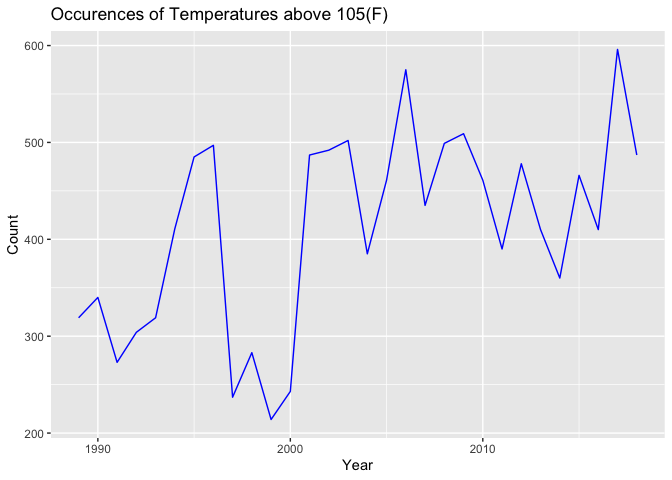
\includegraphics{Final_Project_Submission_files/figure-latex/plot of yearly counts-1.pdf}
\#\#\#It seems that the yearly counts are increasing, but maybe this is
not be completely accurate. Not all stations have the same number of
days during the year that are being reported.

\#\#\#Possibly it is better to take an average by year and plot this,
rather than yearly count. I decide to see how different this plots in
comparison to the yearly count plot.

\begin{Shaded}
\begin{Highlighting}[]
\NormalTok{all_data4 <-}\StringTok{ }\NormalTok{all_data }\OperatorTok
\StringTok{  }\KeywordTok{mutate}\NormalTok{(}\DataTypeTok{above105 =}\NormalTok{ TMAX }\OperatorTok{>=}\StringTok{ }\DecValTok{105}\NormalTok{,}
         \DataTypeTok{above105 =} \KeywordTok{as.numeric}\NormalTok{(above105)) }\OperatorTok
\StringTok{  }\KeywordTok{filter}\NormalTok{(above105}\OperatorTok{==}\DecValTok{1}\NormalTok{) }\OperatorTok
\StringTok{  }\KeywordTok{group_by}\NormalTok{(CITY,YEAR) }\OperatorTok
\StringTok{  }\KeywordTok{summarize}\NormalTok{(}\DataTypeTok{count =} \KeywordTok{n}\NormalTok{()) }\OperatorTok
\StringTok{  }\KeywordTok{group_by}\NormalTok{(YEAR) }\OperatorTok
\StringTok{  }\KeywordTok{summarize}\NormalTok{(}\DataTypeTok{avg =} \KeywordTok{mean}\NormalTok{(count))}
\KeywordTok{head}\NormalTok{(all_data4) }
\end{Highlighting}
\end{Shaded}

\begin{verbatim}
## # A tibble: 6 x 2
##   YEAR    avg
##   <chr> <dbl>
## 1 1989   22.8
## 2 1990   24.3
## 3 1991   18.2
## 4 1992   20.3
## 5 1993   21.3
## 6 1994   41.1
\end{verbatim}

\begin{Shaded}
\begin{Highlighting}[]
\KeywordTok{ggplot}\NormalTok{(all_data4) }\OperatorTok{+}
\StringTok{  }\KeywordTok{geom_line}\NormalTok{(}\DataTypeTok{mapping =} \KeywordTok{aes}\NormalTok{(}\DataTypeTok{x=}\KeywordTok{as.numeric}\NormalTok{(YEAR), }\DataTypeTok{y=}\NormalTok{ avg), }\DataTypeTok{color=} \StringTok{"blue"}\NormalTok{) }\OperatorTok{+}
\StringTok{  }\KeywordTok{labs}\NormalTok{(}\DataTypeTok{title =} \StringTok{"Occurances of Temperatures above 104(F) Per Year"}\NormalTok{, }\DataTypeTok{x =} \StringTok{"Year"}\NormalTok{, }\DataTypeTok{y=} \StringTok{"Average Occurances"}\NormalTok{)}
\end{Highlighting}
\end{Shaded}

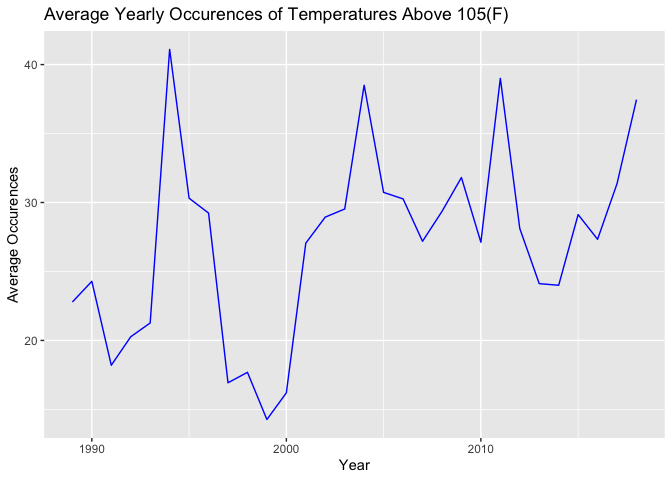
\includegraphics{Final_Project_Submission_files/figure-latex/plot of average yearly counts of extreme tempaverages-1.pdf}

\#\#\#I also wanted to seperate the counts of days each city had with
extreme temperature per year. This shows the days per year for each
city. Some cities experienced more days of extreme temperature per year
than others.Most are pretty consistant over time. I see that some
stations do not provide data for the entire time series. If I were to
repeat this analysis I would try to find station data that provides
temperature measurements for the entire time series.

\begin{Shaded}
\begin{Highlighting}[]
\NormalTok{all_data }\OperatorTok
\StringTok{  }\KeywordTok{mutate}\NormalTok{(}\DataTypeTok{above105 =}\NormalTok{ TMAX }\OperatorTok{>=}\StringTok{ }\DecValTok{105}\NormalTok{,}
         \DataTypeTok{above105 =} \KeywordTok{as.numeric}\NormalTok{(above105)) }\OperatorTok
\StringTok{  }\KeywordTok{filter}\NormalTok{(above105}\OperatorTok{==}\DecValTok{1}\NormalTok{) }\OperatorTok
\StringTok{  }\KeywordTok{group_by}\NormalTok{(CITY,YEAR) }\OperatorTok
\StringTok{  }\KeywordTok{summarize}\NormalTok{(}\DataTypeTok{count =} \KeywordTok{n}\NormalTok{()) }\OperatorTok
\StringTok{  }\KeywordTok{ggplot}\NormalTok{() }\OperatorTok{+}
\StringTok{  }\KeywordTok{geom_line}\NormalTok{(}\KeywordTok{aes}\NormalTok{(}\KeywordTok{as.numeric}\NormalTok{(YEAR),count)) }\OperatorTok{+}
\StringTok{  }\KeywordTok{facet_wrap}\NormalTok{(}\OperatorTok{~}\NormalTok{CITY) }\OperatorTok{+}
\StringTok{  }\KeywordTok{labs}\NormalTok{(}\DataTypeTok{title =} \StringTok{"Number of Days Each City Had Temperatures That Were Above 104(F)"}\NormalTok{, }\DataTypeTok{x=} \StringTok{"Year"}\NormalTok{, }\DataTypeTok{y=} \StringTok{"Count"}\NormalTok{) }\OperatorTok{+}
\StringTok{  }\KeywordTok{facet_wrap}\NormalTok{(}\OperatorTok{~}\NormalTok{CITY)}
\end{Highlighting}
\end{Shaded}

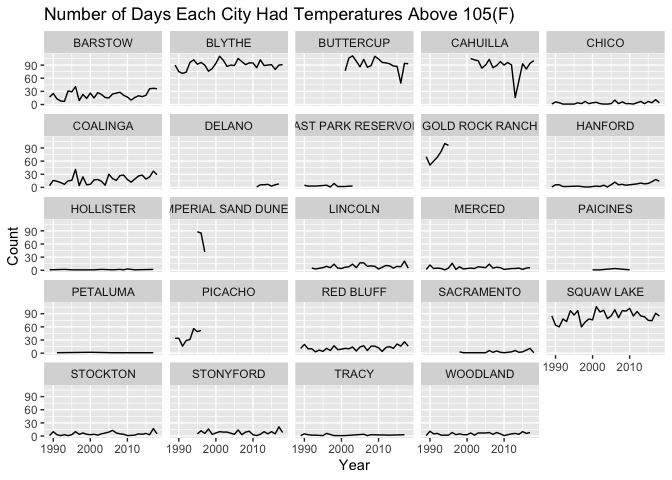
\includegraphics{Final_Project_Submission_files/figure-latex/yearly counts by city-1.pdf}

\#\#Visualizing Location of Reported Temperatures in California \#\#\#I
would now like to create a map of California that shows the location of
each station reporting temperature data. I decided to take the average
number of times there were extreme temperatures in each city, for all of
the years being reported. I then use this to create a color gradient
heat map that shows the cooler and hotter counties. I think that certain
geographic locations of California have more instances of extreme
temperature, on average, than other counties.

\#\#\#Create a new table with the spread of count times that temperature
was above 105 each year in each city.

\begin{Shaded}
\begin{Highlighting}[]
\NormalTok{all_data5 <-}\StringTok{ }\NormalTok{all_data }\OperatorTok
\StringTok{  }\KeywordTok{mutate}\NormalTok{(}\DataTypeTok{above105 =}\NormalTok{ TMAX }\OperatorTok{>=}\StringTok{ }\DecValTok{105}\NormalTok{,}
         \DataTypeTok{above105 =} \KeywordTok{as.numeric}\NormalTok{(above105)) }\OperatorTok
\StringTok{  }\KeywordTok{filter}\NormalTok{(above105}\OperatorTok{==}\DecValTok{1}\NormalTok{) }\OperatorTok
\StringTok{  }\KeywordTok{group_by}\NormalTok{(CITY,YEAR, LATITUDE,LONGITUDE) }\OperatorTok
\StringTok{  }\KeywordTok{summarize}\NormalTok{(}\DataTypeTok{count =} \KeywordTok{n}\NormalTok{()) }\OperatorTok
\StringTok{  }\KeywordTok{group_by}\NormalTok{(CITY, LATITUDE, LONGITUDE) }\OperatorTok
\StringTok{  }\KeywordTok{summarize}\NormalTok{(}\DataTypeTok{avg =} \KeywordTok{mean}\NormalTok{(count)) }
\KeywordTok{head}\NormalTok{(all_data5) }
\end{Highlighting}
\end{Shaded}

\begin{verbatim}
## # A tibble: 6 x 4
## # Groups:   CITY, LATITUDE [6]
##   CITY      LATITUDE LONGITUDE   avg
##   <chr>        <dbl>     <dbl> <dbl>
## 1 BARSTOW       34.9     -117. 21.6 
## 2 BLYTHE        33.6     -115. 74.5 
## 3 BLYTHE        33.6     -115. 28.7 
## 4 BUTTERCUP     32.7     -115. 92.5 
## 5 CAHUILLA      33.0     -115. 89.1 
## 6 CHICO         39.7     -122.  4.83
\end{verbatim}

\begin{Shaded}
\begin{Highlighting}[]
\KeywordTok{ggplot}\NormalTok{(all_data5) }\OperatorTok{+}
\StringTok{  }\KeywordTok{geom_col}\NormalTok{(}\DataTypeTok{mapping=} \KeywordTok{aes}\NormalTok{(}\DataTypeTok{x=}\NormalTok{ CITY, }\DataTypeTok{y =}\NormalTok{ avg)) }\OperatorTok{+}
\StringTok{  }\KeywordTok{labs}\NormalTok{(}\DataTypeTok{title=}\StringTok{"Average Number of Days With Extreme Temperatures Per City"}\NormalTok{, }\DataTypeTok{x=} \StringTok{"City"}\NormalTok{, }\DataTypeTok{y=}\StringTok{"Average Number of Days"}\NormalTok{)}
\end{Highlighting}
\end{Shaded}

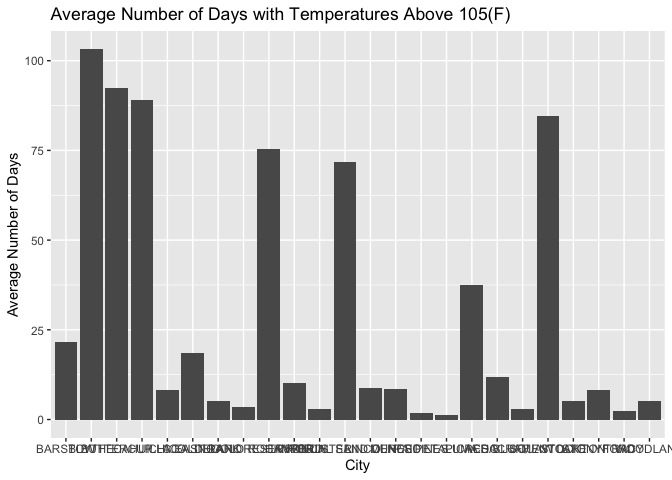
\includegraphics{Final_Project_Submission_files/figure-latex/bar chart of averages-1.pdf}

\#\#\#This histogram is very cluttered along the X axis with city names.
Instead of a histogram I would like to see these cumulative averages per
city plotted on a map of California, because I think these higher
temperatures might be related to region.

\begin{Shaded}
\begin{Highlighting}[]
\NormalTok{ca_map <-}\StringTok{ }\KeywordTok{map_data}\NormalTok{(}\StringTok{"state"}\NormalTok{)}
\NormalTok{ca_map <-}\StringTok{ }\NormalTok{ca_map }\OperatorTok
\StringTok{  }\KeywordTok{filter}\NormalTok{(region }\OperatorTok{==}\StringTok{ "california"}\NormalTok{)}
\end{Highlighting}
\end{Shaded}

\#\#\#This is my map of the points of the station locations that were
used. I used a heat map option to show the comparative averages of each
station location. I can see that there are a few counties that have two
stations reporting. I tried to resolve this error earlier but I am not
sure how to fix this with another method. It is showing that the further
south in California the cities are located, the higher the instances of
extreme temperature.

\begin{Shaded}
\begin{Highlighting}[]
\KeywordTok{ggplot}\NormalTok{() }\OperatorTok{+}
\StringTok{  }\KeywordTok{geom_polygon}\NormalTok{(}\DataTypeTok{data=}\NormalTok{ca_map, }\DataTypeTok{mapping=}\KeywordTok{aes}\NormalTok{(}\DataTypeTok{x =}\NormalTok{ long}\OperatorTok{*}\NormalTok{.}\DecValTok{995}\NormalTok{, }\DataTypeTok{y =}\NormalTok{ lat}\OperatorTok{*}\NormalTok{.}\DecValTok{99}\NormalTok{ ), }\DataTypeTok{inherit.aes =} \OtherTok{FALSE}\NormalTok{, }\DataTypeTok{fill =} \StringTok{"gold"}\NormalTok{, }\DataTypeTok{color =} \StringTok{"blue"}\NormalTok{, }\DataTypeTok{alpha =} \FloatTok{.9}\NormalTok{) }\OperatorTok{+}
\StringTok{  }\KeywordTok{geom_point}\NormalTok{(}\DataTypeTok{data=}\NormalTok{all_data5, }\DataTypeTok{mapping=}\KeywordTok{aes}\NormalTok{(}\DataTypeTok{x =}\NormalTok{ LONGITUDE, }\DataTypeTok{y =}\NormalTok{ LATITUDE, }\DataTypeTok{color=}\NormalTok{avg)) }\OperatorTok{+}\StringTok{ }\KeywordTok{labs}\NormalTok{(}\DataTypeTok{title =} \StringTok{"Location Based Average Counts of Temperatuve Above 104(F)"}\NormalTok{, }\DataTypeTok{x =} \StringTok{"Longitude"}\NormalTok{, }\DataTypeTok{y=} \StringTok{"Latitude"}\NormalTok{)}
\end{Highlighting}
\end{Shaded}

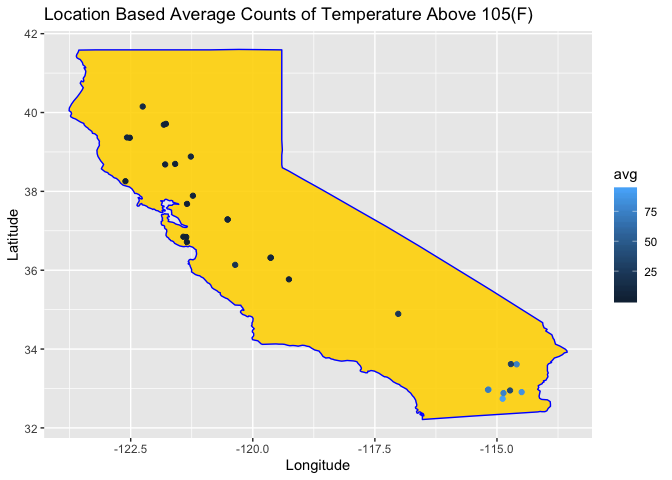
\includegraphics{Final_Project_Submission_files/figure-latex/ca map with station locations-1.pdf}

\#\#Linear Regression and Causality \#\#\#I decided to examine my data
with a linear regression analysis. I want to see the effect that each
variable has on temperature. Examing the regression I see that there is
significant positive temperature change over time. However, my R-squared
value is very low at 0.12, which tells me that I would like to have more
data to strengthen my confidence in my results.

\begin{Shaded}
\begin{Highlighting}[]
\NormalTok{regression_model <-}\StringTok{ }\KeywordTok{lm}\NormalTok{(TMAX }\OperatorTok{~}\StringTok{ }\NormalTok{ELEVATION }\OperatorTok{+}\StringTok{ }\KeywordTok{as.numeric}\NormalTok{(YEAR) }\OperatorTok{+}\StringTok{ }\KeywordTok{factor}\NormalTok{(CITY), }\DataTypeTok{data =}\NormalTok{ all_data)}
\KeywordTok{summary}\NormalTok{(regression_model)}
\end{Highlighting}
\end{Shaded}

\begin{verbatim}
## 
## Call:
## lm(formula = TMAX ~ ELEVATION + as.numeric(YEAR) + factor(CITY), 
##     data = all_data)
## 
## Residuals:
##     Min      1Q  Median      3Q     Max 
## -132.43  -13.05   -0.03   13.42  816.99 
## 
## Coefficients:
##                                   Estimate Std. Error t value Pr(>|t|)    
## (Intercept)                     -28.052509   9.536666  -2.942  0.00327 ** 
## ELEVATION                        -0.003974   0.006158  -0.645  0.51866    
## as.numeric(YEAR)                  0.055509   0.004865  11.411  < 2e-16 ***
## factor(CITY)BLYTHE                6.331809   3.608644   1.755  0.07933 .  
## factor(CITY)BUTTERCUP             7.569596   3.776108   2.005  0.04501 *  
## factor(CITY)CAHUILLA              6.890490   3.661864   1.882  0.05988 .  
## factor(CITY)CHICO                -7.704933   3.754255  -2.052  0.04014 *  
## factor(CITY)COALINGA             -1.590293   2.917859  -0.545  0.58574    
## factor(CITY)DELANO               -4.868650   3.631662  -1.341  0.18005    
## factor(CITY)EAST PARK RESERVOIR  -7.700943   1.915275  -4.021 5.80e-05 ***
## factor(CITY)GOLD ROCK RANCH       6.658700   3.263003   2.041  0.04129 *  
## factor(CITY)HANFORD              -5.923064   3.713193  -1.595  0.11068    
## factor(CITY)HOLLISTER           -10.610299   3.527472  -3.008  0.00263 ** 
## factor(CITY)IMPERIAL SAND DUNES   8.940575   3.804984   2.350  0.01879 *  
## factor(CITY)LINCOLN              -6.216143   3.799659  -1.636  0.10185    
## factor(CITY)LORAINE              -8.100243   3.784220  -2.141  0.03231 *  
## factor(CITY)MERCED               -6.010159   3.884694  -1.547  0.12183    
## factor(CITY)PAICINES            -10.585135   2.481356  -4.266 1.99e-05 ***
## factor(CITY)PETALUMA            -12.837266   4.135800  -3.104  0.00191 ** 
## factor(CITY)PICACHO               3.763323   2.599561   1.448  0.14771    
## factor(CITY)RED BLUFF            -6.560271   3.511412  -1.868  0.06173 .  
## factor(CITY)SACRAMENTO           -8.488989   4.137062  -2.052  0.04018 *  
## factor(CITY)SQUAW LAKE            7.015731   3.610846   1.943  0.05202 .  
## factor(CITY)STOCKTON             -7.621160   4.124082  -1.848  0.06461 .  
## factor(CITY)STONYFORD            -6.303026   1.932211  -3.262  0.00111 ** 
## factor(CITY)TRACY                -5.548014   3.920422  -1.415  0.15702    
## factor(CITY)WOODLAND             -7.138162   4.047597  -1.764  0.07781 .  
## ---
## Signif. codes:  0 '***' 0.001 '**' 0.01 '*' 0.05 '.' 0.1 ' ' 1
## 
## Residual standard error: 16.37 on 198737 degrees of freedom
## Multiple R-squared:  0.122,  Adjusted R-squared:  0.1219 
## F-statistic:  1062 on 26 and 198737 DF,  p-value: < 2.2e-16
\end{verbatim}

\#\#Other Plot of Temperature Data \#\#\#I have taken the yearly average
number of days of extreme temperature in all the cities per year with
95\% confidence intervals. Signifcance is indicated by shifts beyond
95\% confidence range for each year.

\begin{Shaded}
\begin{Highlighting}[]
\NormalTok{all_data }\OperatorTok
\StringTok{  }\KeywordTok{mutate}\NormalTok{(}\DataTypeTok{above105 =}\NormalTok{ TMAX }\OperatorTok{>=}\StringTok{ }\DecValTok{105}\NormalTok{,}
         \DataTypeTok{above105 =} \KeywordTok{as.numeric}\NormalTok{(above105)) }\OperatorTok
\StringTok{  }\KeywordTok{filter}\NormalTok{(above105}\OperatorTok{==}\DecValTok{1}\NormalTok{) }\OperatorTok
\StringTok{  }\KeywordTok{group_by}\NormalTok{(CITY,YEAR) }\OperatorTok
\StringTok{  }\KeywordTok{summarize}\NormalTok{(}\DataTypeTok{freq =} \KeywordTok{n}\NormalTok{()) }\OperatorTok
\StringTok{  }\KeywordTok{group_by}\NormalTok{(YEAR) }\OperatorTok
\StringTok{  }\KeywordTok{summarize}\NormalTok{(}\DataTypeTok{avg =} \KeywordTok{mean}\NormalTok{(freq),}
            \DataTypeTok{stdev =} \KeywordTok{sd}\NormalTok{(freq),}
            \DataTypeTok{upper =}\NormalTok{ avg }\OperatorTok{+}\StringTok{ }\NormalTok{(stdev}\OperatorTok{*}\FloatTok{1.96}\OperatorTok{/}\KeywordTok{sqrt}\NormalTok{(}\KeywordTok{n}\NormalTok{())),}
            \DataTypeTok{lower =}\NormalTok{ avg }\OperatorTok{-}\StringTok{ }\NormalTok{(stdev}\OperatorTok{*}\FloatTok{1.96}\OperatorTok{/}\KeywordTok{sqrt}\NormalTok{(}\KeywordTok{n}\NormalTok{()))}
\NormalTok{            ) }\OperatorTok
\StringTok{  }\KeywordTok{ggplot}\NormalTok{() }\OperatorTok{+}
\StringTok{  }\KeywordTok{geom_point}\NormalTok{(}\KeywordTok{aes}\NormalTok{(}\DataTypeTok{x =} \KeywordTok{as.character}\NormalTok{(YEAR), }\DataTypeTok{y =}\NormalTok{ avg)) }\OperatorTok{+}
\StringTok{  }\KeywordTok{geom_linerange}\NormalTok{(}\KeywordTok{aes}\NormalTok{(}\DataTypeTok{x =} \KeywordTok{as.character}\NormalTok{(YEAR), }\DataTypeTok{ymax =}\NormalTok{ upper, }\DataTypeTok{ymin =}\NormalTok{ lower)) }\OperatorTok{+}
\StringTok{  }\KeywordTok{labs}\NormalTok{(}\DataTypeTok{title =} \StringTok{"Yearly Average of Days Temperatures Above 104(F) Across Cities"}\NormalTok{, }\DataTypeTok{x=} \StringTok{"Year"}\NormalTok{, }\DataTypeTok{y=} \StringTok{"Average Number of Days"}\NormalTok{)}
\end{Highlighting}
\end{Shaded}

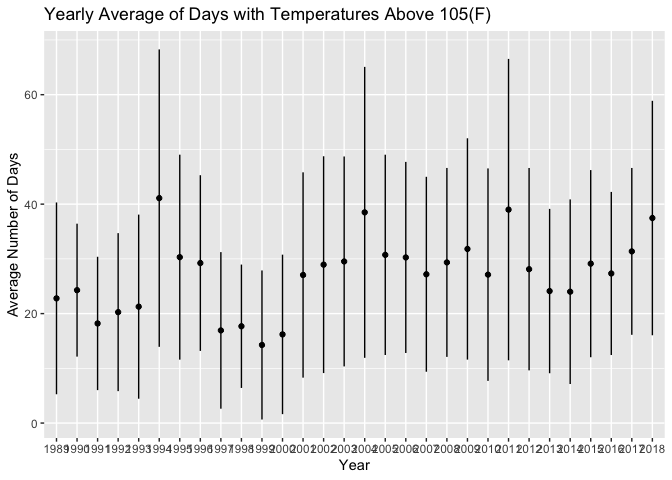
\includegraphics{Final_Project_Submission_files/figure-latex/other plots of data-1.pdf}


\end{document}
